%
% Slide
%
\begin{frame}
  \frametitle{A Search Algorithm}
  \begin{minipage}{0.55\textwidth}
    \begin{itemize}
      \item \textbf{Input:} (1) An array of numbers and (2) number for which we're searching.\\
      \item \textbf{Output:} Whether or not the number exists in the list of numbers.\\
      \item \textbf{Algorithm:} \\
      \begin{enumerate}
        \item Look at first item.
        \item Check if it's the item we're looking for.
        \item If it's the item we're looking for stop otherwise go to next item.
        \item Repeat steps 2 \& 3 if there are still items in the list.
      \end{enumerate}
    \end{itemize}
  \end{minipage}
  \hfill
  \begin{minipage}{0.39\textwidth}
    \textbf{Searching Number:} 4\\
    \vspace{0.1cm}\\
    \textbf{Input List:}\\
    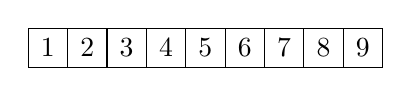
\begin{tikzpicture}
      \draw[draw=black] (0,0) rectangle (.5,.5) node[pos=0.5] {1};
      \draw[draw=black] (.5,0) rectangle (1,.5) node[pos=0.5] {2};
      \draw[draw=black] (1,0) rectangle (1.5,.5) node[pos=0.5] {3};
      \draw[draw=black] (1.5,0) rectangle (2,.5) node[pos=0.5] {4};
      \draw[draw=black] (2,0) rectangle (2.5,.5) node[pos=0.5] {5};
      \draw[draw=black] (2.5,0) rectangle (3,.5) node[pos=0.5] {6};
      \draw[draw=black] (3,0) rectangle (3.5,.5) node[pos=0.5] {7};
      \draw[draw=black] (3.5,0) rectangle (4,.5) node[pos=0.5] {8};
      \draw[draw=black] (4,0) rectangle (4.5,.5) node[pos=0.5] {9};
    \end{tikzpicture}
  \end{minipage}
\end{frame}

\begin{frame}
  \centering
  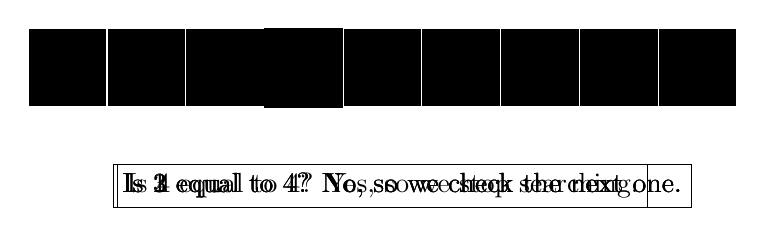
\begin{tikzpicture}
    \pgfmathtruncatemacro{\N}{4}
    \pgfmathtruncatemacro{\asize}{9}
    \foreach \n in {1,2,...,\N}{
      \onslide<\n>{

        \foreach \i in {1,2,3,...,\asize}{
          \ifnum\i=\n
            \draw[draw=black] (\i-1,0) rectangle (\i,1) node[pos=0.5] {\i};
          \else
            \draw[draw=white, fill=black] (\i-1,0) rectangle (\i,1);
          \fi
        }

        \ifnum\n=\N
          \node[draw] at (4.5, -1) {Is \n\ equal to \N? Yes, so we stop searching.};
        \else
          \node[draw] at (4.75, -1) {Is \n\ equal to \N? No, so we check the next one.};
        \fi
      }
    }
  \end{tikzpicture}
\end{frame}

